\documentclass[final,12pt]{beamer}

\mode<presentation> {
  \usetheme{Custom}
}

\usepackage[english]{babel}
\usepackage[orientation=portrait,size=a0,scale=1.4,debug]{beamerposter}
\usepackage{adjustbox}
\usepackage{algpseudocode}
\usepackage{amsmath,amsthm,amssymb,latexsym}
\usepackage{hyperref}
\usepackage{listings}
\usepackage{times}

\lstset{
  language=C,
  keywordstyle=\color{blue}
}

\boldmath

\hypersetup{
  colorlinks,
  linkcolor=,
  urlcolor=blue
}

\makeatletter
\renewcommand{\ALG@beginalgorithmic}{\small}
\makeatother

\title{Implementation of Cache Management Algorithms in DM-Cache}
\author{Jesus Ramos (jramo028@fiu.edu)}
\institute[FIU]{Florida International University}
\date{}

\begin{document}
\begin{frame}{}

  \begin{columns}
    \begin{column}{.33\linewidth}
      \begin{block}{\large Problem Statement}
        Choosing an effective cache management policy for your caches can make a
        huge difference when it comes to application performance. This is
        especially true for I/O intensive applications where a miss can take
        anywhere from 6 milliseconds to even a couple of seconds if the request
        goes to an idle disk. Placing some of this data on a local solid state
        drive can improve I/O response time from the data read from the SSD to
        somewhere between 500 microseconds and 1 millisecond.
      \end{block}
    \end{column}

    \begin{column}{.33\linewidth}
      \begin{block}{\large Current Solutions}
        DM-Cache currently implements a hash based eviction policy. Rather than
        using recency information eviction is done based on hash
        collisions. DM-Cache uses the kernel function \texttt{hash\_long()} to
        generate a 64 bit hash value based on the sector number of the
        request. When two requests map to the same block the last one is
        invalidated and flushed if need be and then evicted to make room for the
        new block.
      \end{block}
    \end{column}

    \begin{column}{.33\linewidth}
      \begin{block}{\large Objectives}

        \begin{itemize}
          \item Make DM-Cache more flexible when it comes to cache management
          \item Allow for implementation of other cache management algorithms
          \item Update the existing code base to a more recent kernel
          \item Lower the memory footprint of DM-Cache
        \end{itemize}

      \end{block}
    \end{column}

  \end{columns}

  \begin{block}{\large Design and Implementation}

    \begin{columns}

      \begin{column}{.01\textwidth}
      \end{column}

      \begin{column}{.33\textwidth}
        \begin{algorithmic}
  \State $block \gets$ look-up requested block in $radix\_tree$
  \If {$block$ is not cached}
    \If {$cache$ is full}
      \State evict from tail of $lru\_list$
    \EndIf
    \State initialize new $block$
    \State insert $block$ into $radix\_tree$
  \EndIf
  \State move $block$ to head of $lru\_list$
\end{algorithmic}

        \centering \small Pseudo-code for DM-Cache using LRU (Least Recently
        Used) cache eviction algorithm
      \end{column}

      \begin{column}{.33\textwidth}
        \begin{algorithmic}
  \State $block \gets$ look-up requested block in $radix\_tree$
  \If {$block$ is not cached}
    \If {$cache$ is full}
      \State evict from tail of $lfu\_list$
    \EndIf
    \State initialize new $block$
    \State insert $block$ into $radix\_tree$
    \State insert $block$ at tail of $lfu\_list$ with $hit\_count$ of $1$
  \Else
    \State $block.hit\_count \gets block.hit\_count + 1$
    \State $next\_block \gets$ adjacent entry of $block$ from $lfu\_list$
    \If {$block.hit\_count \geq next\_block.hit\_count$}
      \State swap $block$ and $next\_block$ in place
    \EndIf
  \EndIf
\end{algorithmic}


        \centering \small Pseudo-code for DM-Cache using LFU (Least Frequently
        Used) cache eviction algorithm
      \end{column}

      \begin{column}{.33\textwidth}

        \textbf{Policies:} \\

        Least Recently Used (LRU) and Least Frequently Used (LFU) were chosen as
        the eviction policies to implement as they are the most popular eviction
        policies and can be proven to outperform others in the most cases. To
        the left the algorithms are detailed in the context of how they perform
        in DM-Cache.

      \end{column}

    \end{columns}

    \textbf{Updating the Code-base:} \\

    The implementation of DM-Cache used as a base was written for kernel
    2.6.19. This version is pretty outdated as the new stable kernel version is
    2.6.36 so the code-base was updated to this newer version. The documentation
    for the device mapper functionality in the kernel hasn't been updated (and
    as of writing even in 3.0 the documentation is still out of date) so to
    figure out the changes I had to delve into the code. One of the most notable
    and hard to track changes was the removal of the \texttt{dm\_io\_get()} and
    \texttt{dm\_io\_put()} functions. Their removal was not documented although
    after some tracking I found that they were replaced by a \texttt{struct
      dm\_io\_client} and two new functions \texttt{dm\_io\_client\_create()}
    and \texttt{dm\_io\_client\_destroy()}. This allows modules that make use of
    the device mapper to allocate private memory pools and block I/O sets so
    that they do not contend for memory.

    % Device mapper changed its memory request scheme for allocating memory for
    % I/O requests that must pass through the device mapper. The old method for
    % accomplishing this involves requesting pages through the
    % \texttt{dm\_io\_get()} function and then later using \texttt{dm\_io\_put()}
    % to release the pages when they are no longer needed. These functions were
    % removed in later kernels and replaced with a structure called
    % \texttt{dm\_io\_client}. This allowed many users of device mapper to share
    % pages instead of having to make separate requests for each device mapper
    % pseudo-device. Requests are now done by creating a client by calling
    % \texttt{dm\_io\_client\_create()} in much the same way the previous function
    % was called and its counterpart \texttt{dm\_io\_client\_destroy()} to release
    % the used pages.

    \vspace{\baselineskip}

    \textbf{Implementation:} \\

    The hash table in DM-Cache was replaced with \texttt{struct
      radix\_tree\_root} ordered by request sector numbers as well as the
    addition of a \texttt{struct list\_head} to maintain the LRU and LFU lists
    such that candidates for eviction are always at the tail of the list. The
    eviction policy was also modified so that whenever all available blocks have
    been filled one is pulled from the tail of the list, invalidated, and
    replaced with the most recently requested block.

    \vspace{\baselineskip}

    While the implementation sounds straight forward it required changes to
    around 1200 lines of code. This is due to the fact that the hash table was
    always accessed directly so every reference to that had to be changed. There
    was also additional code to be written that had to handle the new policies
    compounded on top of the changes required to make the module functional in
    version 2.6.36 of the kernel.

  \end{block}

  \begin{columns}

    \begin{column}{.5\linewidth}
      \begin{block}{\large Screenshots}
        \centering
        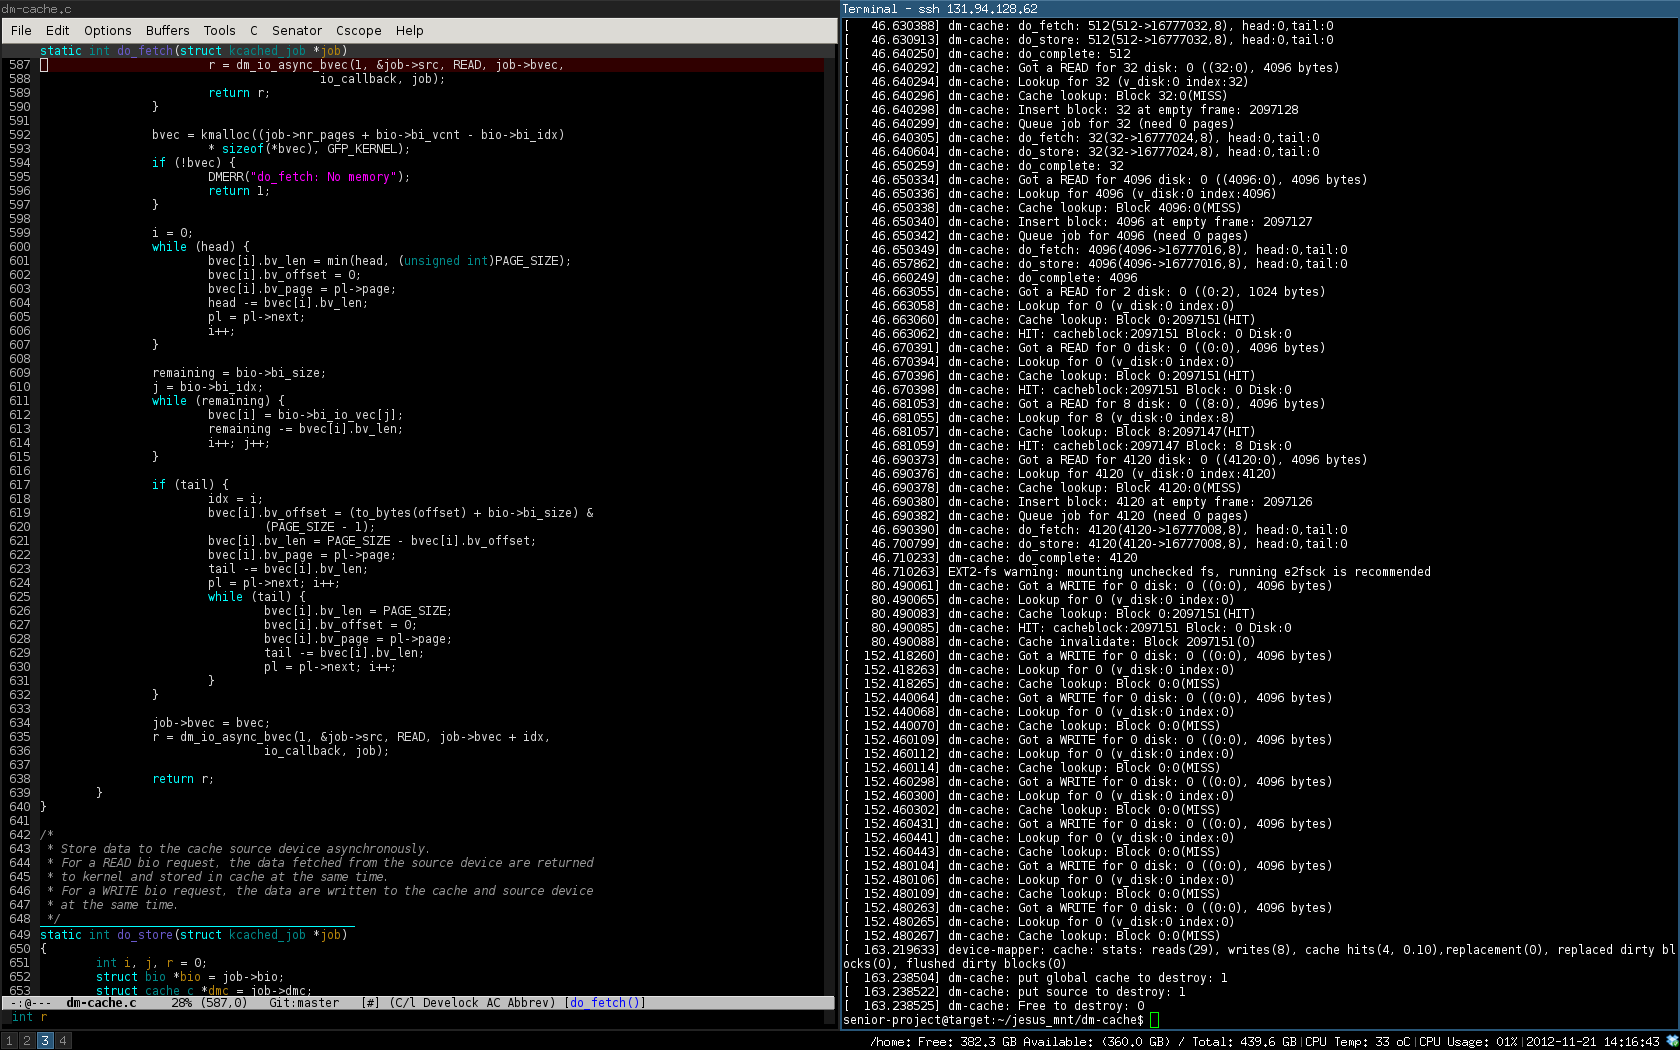
\includegraphics[width=.97\textwidth]{../images/screenshot.png}
      \end{block}
    \end{column}

    \begin{column}{.5\linewidth}
      \begin{block}{\large Testing}

        Testing was done using a virtual machine using an 8GB cache size. To
        exercise the cache eviction algorithms a test file size of 16GB was
        used. The tests that were performed were sequential writes, random
        writes, sequential reads, and random reads all using a 16GB file. To
        test that the cache was not losing or corrupting any blocks an original
        copy of the file was kept and the \texttt{diff} utility was run to check
        for inconsistencies.

        \vspace{\baselineskip}

        The code for this project can be found at:
        \url{https://github.com/jesus-ramos/senior-project}

        More information on DM-Cache can be found at:
        \url{https://github.com/mingzhao/dm-cache} \\
        and at: \\
        \url{http://visa.cs.fiu.edu/}

      \end{block}
    \end{column}

  \end{columns}

  % unneeded for now
  % \begin{block}{\large References}
  % \end{block}

\end{frame}
\end{document}